% THIS IS SIGPROC-SP.TEX - VERSION 3.1
% WORKS WITH V3.2SP OF ACM_PROC_ARTICLE-SP.CLS
% APRIL 2009
%
% It is an example file showing how to use the 'acm_proc_article-sp.cls' V3.2SP
% LaTeX2e document class file for Conference Proceedings submissions.
% ----------------------------------------------------------------------------------------------------------------
% This .tex file (and associated .cls V3.2SP) *DOES NOT* produce:
%       1) The Permission Statement
%       2) The Conference (location) Info information
%       3) The Copyright Line with ACM data
%       4) Page numbering
% ---------------------------------------------------------------------------------------------------------------
% It is an example which *does* use the .bib file (from which the .bbl file
% is produced).
% REMEMBER HOWEVER: After having produced the .bbl file,
% and prior to final submission,
% you need to 'insert'  your .bbl file into your source .tex file so as to provide
% ONE 'self-contained' source file.
%
% Questions regarding SIGS should be sent to
% Adrienne Griscti ---> griscti@acm.org
%
% Questions/suggestions regarding the guidelines, .tex and .cls files, etc. to
% Gerald Murray ---> murray@hq.acm.org
%
% For tracking purposes - this is V3.1SP - APRIL 2009

\documentclass{acm_proc_article-sp}
\usepackage{filecontents}

\begin{document}
\title{Latent Dirichlet Allocation as a Twitter Hashtag Recommender System
	\titlenote{There are no legal restrictions! Break all the rules! We don't own this, and wouldn't even dare claim it if our lives depended on it. Plagiarize to your heart's desire, but maybe hook us up with a job interview if you think we had some good ideas in here.}}



\numberofauthors{2} 
\author{
\alignauthor
Brian Gillespie\\
       \affaddr{Northeastern University}\\
       \affaddr{Seattle, WA}\\
       \email{bng1290@gmail.com}
\alignauthor
Shailly Saxena\\
       \affaddr{Northeastern University}\\
       \affaddr{Seattle, WA}\\
       \email{saxena.sha@husky.neu.edu}
}

\date{26 March 2016}



\maketitle
\begin{abstract}
\hspace*{5mm}In this paper, we investigate an unsupervised approach to hashtag recommendation, to aid in the classification of tweets. Two corpora were generated from a sample of tweets collected from September 2009 to January 2010. The first corpus was composed simply of individual tweets, and the second corpus was made by aggregating tweets by UserID into what is referred to as the USER PROFILE model. Latent Dirichlet Allocation(LDA) was used to generate topic distributions for each corpus, and then Collapsed Gibbs Sampling was used to generate topic distributions for new test tweets. By sampling a topic from each test tweet, and then sampling one of the top terms from that topic, a set of words can be selected as recommended hashtags. This recommendation process was applied to several example tweets, and the relevancy of the suggested hashtags were evaluated by human observers. The results of this would be briefly mentioned here if there were any.
\end{abstract}

\keywords{Twitter, LDA, topic modeling, NLP, social media} 

\section{Introduction}
\hspace*{5mm}Twitter is an amazing source of text data, both in content and quantity. With over 305 million monthly active users across the globe, there are a wide variety of subjects being discussed. Cataloging this data, and finding ways to make it more search-able is very desirable, as this data can be an effective resource for business knowledge and studying social trends. Hashtags appear as the natural categorization index for tweets, however since only 8\% of tweets contain a hashtags, they cannot be used as a direct categorization for all tweets. Compounding this issue, there are no prescribed hashtags; any sequence of characters can be a hashtag as long as it has a \# in front of it. A hashtag recommendation system can be implemented to encourage users to utilize more hashtags, and to provide a more consolidated hashtag base for tweet categorization. But in order to avoid prescribing hashtags, and thus limiting the free expression of Twitter users, it is more reasonable to generate the suggested hashtags from the content of Twitter itself. This has the added gain of providing an adaptable system that can develop alongside the vocabulary and interests of the Twitter user base.

\section{Related Work}
\hspace*{5mm}Although there has been much research in the structure and dynamics of microblogging networks, and many insights have been gained by looking into how users interact with one another and with the world, the area of hashtag recommendations is still not explored enough. Providing hashtags is an important feature of Twitter for they aid in classification and easy retrieval of tweets and <<something>>.\\
\hspace*{5mm}There have been recent developments in hashtag recommendation approaches to Twitter data such as Zangerle et al. \cite{zangerle2011recommending} and Kywe, Hoang, et al.\cite{kywe2012recommending} where recommendations are made on the basis of similarity. These similarities can be of tweet content or users. Zangerle et al. \cite{zangerle2011recommending} analyzed three different ways of tweet recommendations. They rank the hashtags based on the overall popularity of the tweet, the popularity within the most similar tweets, and the most similar tweets. Out of these, the third approach out-performs the rest. On the other hand, Mazzia and Juett \cite{mazzia2009suggesting} use a naive Bayes model to determine the relevance of hashtags to an individual tweet. Since these methods do not take into consideration, the personal preferences of the user, Kywe et al. \cite{kywe2012recommending} suggest recommending hashtags incorporating similar users along with similar tweets and thus achieving more than 20\% accuracy than the above stated methods.\\
\begin{table*}[ht]
	\caption{Twitter Sample Sep 2009 to Jan 2010}
	\centering
	\begin{tabular}{c c}   
		\hline\hline\rule{0pt}{2ex}
		UserID & Tweet \\
		\hline\rule{0pt}{3ex}
		66 & For all the everything you've brought to my internet life \#mathowielove \\
		53717680 & What's good Tweeps this Friday \\
		16729208 &"I bet you all thought Bert \& Ernie were just roommates!" \\ 
		86114354 & @miakhyrra take me with you! lol \\ [1ex] 
		\hline 
	\end{tabular}
	\label{table:sample} % refer to this table in the text
\end{table*}
\hspace*{5mm}One of the drawbacks of these approaches is that they rely on existing hashtags to recommend the new ones. Since, the current number of hashtags is already very low and very few of them are hardly ever repeated, using these hashtags will not improve classification of tweets.  \cite{godin2013using} Godin et. al took these into consideration and applied LDA model which was trained to cluster tweets in a number of topics from which keywords can be suggested for new tweets. In this paper, we extend Godin et. al \cite{godin2013using} by incorporating \textit{user profile} approach as suggested in \cite{hong2010empirical} . In user this approach, tweets were aggregated by the User IDs of their authors, and a new set of documents was created where each document is a \textit{user profile} of a unique user id and his or her combined set of tweets.\\
\hspace*{5mm}In this paper, we explore some of the more promising approaches to hashtags recommendations in tweets, and investigate their implications to further research into developing a more successful Twitter hashtags recommendations using topic modeling. Due to the success of the \textit{user profile} approach, we will employ and evaluate this method, to further investigate its effectiveness.\\

\section{Dataset and Preprocessing}
\hspace*{5mm}The datasets used were obtained from Cheng, Caverlee, and Lee \cite{cheng2010content}. In order to reduce noise in the text data, a set of stop words were removed from the tweet bodies, the remaining words were then stemmed, and any hyperlinks were also removed. A bag of words model was created, and TF-IDF vectors were generated. For the \textit{user profile} LDA approach \cite{hong2010empirical} and the Twitter-LDA model \cite{zhao2011comparing}, the vectors were aggregated based on user IDs. We also processed each tweet for the documents ``as-is'' for the Twitter-LDA model. The training and tests datasets were merged, and then re-partitioned to prepare for 10-fold cross-validation.


\subsection{The Dataset}
\hspace*{5mm}The training dataset from Cheng, Caverlee, and Lee \cite{cheng2010content}, contains 3,844,612 tweets from 115,886 Twitter users over the time period of September 2009 to January 2010. The test set, also from \cite{cheng2010content}, contains 5,156,047 tweets from 5,136 Twitter users over the same time period. In general, tweets contain between 1 and 20 words, with an average of 7 words per tweet. A smaller proportion of the tweets contained more than 20 words as seen in Figure 1. Each line of the dataset contains a unique user ID and tweet ID, text content, and a timestamp. The text content of each tweet is limited to 140 characters, and can contain references to other users of the form @username, as well as popular \#hashtags. Many tweets also include hyperlinks which are often passed through URL shorteners (e.g. http://goo.gl/uLLAe). The implications of these more anomalous text instances are considered in the next section.\\
\hspace*{5mm}An additional document corpus was generated from each dataset by aggregating tweets by user ID. This reduction is referred to as the \textit{user profile} model \cite{hong2010empirical}. After aggregation, the corpus contained a total of 115,886 documents. Data preprocessing was performed on both of these corpora, and is described in the next section.
 
\subsection{Data Preprocessing and Reduction}
\hspace*{5mm}Due to the unconventional vocabulary in tweets and the large amount of noise inherent in such a diverse set of text, we decided to perform several data preprocessing steps. A regular expression was used to remove any non-latin characters and any URL links, as URL links are generated randomly and cannot be easily related to a topic. After pruning the tweet contents, the text was tokenized, stop words were removed, and the remaining tokens were stemmed using the Porter Stemming library from the Natural Language Toolkit (NLTK). The prepared corpus of tweets was then converted to a set of Term Frequency (TF) vectors, using the corpora library from gensim. \\
We noticed that many tweets contained excessive repetition of words (for instance one tweet read: "@jester eh eh eh eh eh eh eh eh eh..."), so in order to reduce any bias towards overused words in the data we removed words appearing over 5 times in a tweet, as well as using the TF-IDF model to reduce emphasis on such words. To reduce bias to common words across the corpus, we removed terms appearing in over 70\% of the documents as per \cite{zhao2011comparing}. As seen in Figure 2, before preprocessing the data was dominated by common words that do not confer much meaning (e.g get, u, just, one). After preprocessing, however, we begin to see more meaningful words (e.g people, twitter, home, blog in Figure 3). After preprocessing, there were 26,542,006 total words and 184,002 unique words in the vocabulary.\\


\begin{figure}[ht]
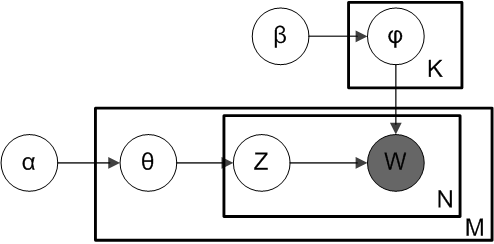
\includegraphics[scale=0.48]{figs/Smoothed_LDA}
\caption{Plate Diagram of LDA.}
\end{figure}

\section{Model and Methodology}
\hspace*{5mm}Latent Dirichlet Allocation, first proposed by Blei, Ng, and Jordan \cite{blei2003latent} is a generative probabilistic model, that supposes each document in a corpus is generated from a smaller, hidden set of topics. Each word in a document is drawn from a topic, making every document a mixture of samples from a variety of different topics. There are multiple ways of estimating these hidden topics, including Hidden Markov Monte Carlo techniques such as Collapsed Gibbs Sampling \cite{griffiths2002gibbs}, or with a stochastic gradient descent method such as in \cite{hoffman2010online}. In this paper we utilized the latter, and the details of our topic model generation are discussed in the next section.\\
\hspace*{5mm}For the purpose of hashtag recommendation, we first need to see which topics are most represented by a new tweet. We then propose that the most significant words from within those  strongly related topics will provide a more general representation of the message contained in a given tweet. So essentially for each new test tweet, we sample from the top topics in that tweet, and we recommend a hashtag from the top most representative words in that topic. In this way, we are recommending topics that also reflect the social component of Twitter. Since the topics we find are driven by the tweets themselves, our recommendations serve as an approximation of the connections between what users are talking about.\\

\subsection{Getting a Topic Model}
\hspace*{5mm}In order to generate our topic model, we utilized the LDAModel package from gensim. This package uses the \textit{onlineldavb.py} algorithm that was proposed in \cite{hoffman2010online}. This is an online, constant memory implementation of the LDA algorithm, which allowed us to process a rather large dataset with limited resources. This package processes the documents in mini batches, and we chose our batch size to be the default, 2,000. The key parameters kappa and tau as mentioned in \cite{hoffman2010online} were kept at 0.5 and 1.0, respectively, as these values performed best in their performance analyses. Symmetric priors were also kept for the topic-to-word and document-to-topic distributions; these priors can be tweaked in order to boost certain topics or terms. Finally, our choices for number of topics were chosen based on the more successful results seen in \cite{hong2010empirical}. For the per tweet based corpus we chose topic sizes of 50, 100, and 200 in keeping with \cite{godin2013using}. However for the \textit{user profile} model we turned to the experiments by Hong, et. al., who determined that this approach tends to favor lower topic sizes, and in their case a size of 40 performed best. For our own \textit{user profile} implementation we used topic sizes of 20, 40, 70, and 100.\\ 
\hspace*{5mm}Since several models were created, it is informative to see if our various approaches have had much of an effect on the final model. In order to compare the similarity of our topic distributions, we plan to calculate the Jensen-Shannon divergence between the topic matrices generated by running LDA for each of our selected topic sizes and training corpora. By comparing these similarity measures, we can see if there was any effect with using the \textit{user profile} model, or by changing the topic sizes. From here elaborate the results of our comparisons.\\
​
\subsection{Hashtag Recommendation}
\hspace*{5mm}In order to provide recommendations for a new tweet, we first decided to do some quick preliminary preprocessing by removing any user-added hashtags, references to other users, URL links, and non-latin characters. From here, we can convert this new document into its TF-IDF representation and merge this into our existing dictionary. We used the LDA model generated previously to infer the topics from which each word in the tweet is drawn. This can also be done using gensim; by querying the generated model, LDAModel will return the distribution of topics and their respective posterior probabilities for a given document. Using the belief that each document represents some mixture of topics, we can sample the most strongly correlated topics from a new tweet. Next, we select one of these strong topics, and recommend a hashtag from the set of words that make up that topic. In this experiment, we decided to only select from the words that most strongly represent their topics, in the hopes that this will strengthen the relevance of our suggestions.\\

\section{Evaluation}
\hspace*{5mm}In order to evaluate the quality of recommendations from our model, we decided to make a  simple web app, where a user can write out a tweet and the number of hashtags they'd like, and see our recommendations. We intend to provide this setup to several human testers, who will evaluate whether a given hashtag is relevant to their submission or not.\\


%\begin{figure*}[ht]
%	\centering
%	\includegraphics[width=\textwidth, height=75mm]{figs/topwordsorig}
%	\caption{Original barchart of the top 20 words and their counts.}
%	\includegraphics[width=\textwidth, height=75mm]{figs/topwords}
%	\caption{Barchart of the top 20 words and their counts after preprocessing.}
%\end{figure*}


\begin{filecontents}{jobname.bib}
@incollection{zhao2011comparing,
	title={Comparing twitter and traditional media using topic models},
	author={Zhao, Wayne Xin and Jiang, Jing and Weng, Jianshu and He, Jing and Lim, Ee-Peng and Yan, Hongfei and Li, Xiaoming},
	booktitle={Advances in Information Retrieval},
	pages={338--349},
	year={2011},
	publisher={Springer}
}
@inproceedings{hong2010empirical,
	title={Empirical study of topic modeling in twitter},
	author={Hong, Liangjie and Davison, Brian D},
	booktitle={Proceedings of the first workshop on social media analytics},
	pages={80--88},
	year={2010},
	organization={ACM}
}
@inproceedings{cheng2010content,
	title={You Are Where You Tweet: A Content-Based Approach to Geo-locating Twitter Users},
	author={Z. Cheng, J. Caverlee, and K. Lee},
	booktitle={Proceeding of the 19th ACM Conference on Information and Knowledge Management (CIKM)},
	month={October},
	year={2010}
}
@article{blei2003latent,
	title={Latent dirichlet allocation},
	author={Blei, David M and Ng, Andrew Y and Jordan, Michael I},
	journal={the Journal of machine Learning research},
	volume={3},
	pages={993--1022},
	year={2003},
	publisher={JMLR. org}
}
@inproceedings{hoffman2010online,
	title={Online learning for latent dirichlet allocation},
	author={Hoffman, Matthew and Bach, Francis R and Blei, David M},
	booktitle={advances in neural information processing systems},
	pages={856--864},
	year={2010}
}
@incollection{kywe2012recommending,
	title={On recommending hashtags in twitter networks},
	author={Kywe, Su Mon and Hoang, Tuan-Anh and Lim, Ee-Peng and Zhu, Feida},
	booktitle={Social Informatics},
	pages={337--350},
	year={2012},
	publisher={Springer}
}
@article{mazzia2009suggesting,
	title={Suggesting hashtags on twitter},
	author={Mazzia, Allie and Juett, James},
	journal={EECS 545m, Machine Learning, Computer Science and Engineering, University of Michigan},
	year={2009}
}
@inproceedings{zangerle2011recommending,
	title={Recommending\#-tags in twitter},
	author={Zangerle, Eva and Gassler, Wolfgang and Specht, Gunther},
	booktitle={Proceedings of the Workshop on Semantic Adaptive Social Web (SASWeb 2011). CEUR Workshop Proceedings},
	volume={730},
	pages={67--78},
	year={2011}
}
@inproceedings{li2011twitter,
	title={Twitter hash tag prediction algorithm},
	author={Li, Tianxi and Wu, Yu and Zhang, Yu},
	booktitle={ICOMP’11-The 2011 International Conference on Internet Computing},
	year={2011}
}
@inproceedings{godin2013using,
	title={Using topic models for twitter hashtag recommendation},
	author={Godin, Fr{\'e}deric and Slavkovikj, Viktor and De Neve, Wesley and Schrauwen, Benjamin and Van de Walle, Rik},
	booktitle={Proceedings of the 22nd international conference on World Wide Web companion},
	pages={593--596},
	year={2013},
	organization={International World Wide Web Conferences Steering Committee}
}
@article{griffiths2002gibbs,	
	title={Gibbs sampling in the generative model of latent dirichlet allocation},
	author={Griffiths, Tom},
	year={2002},
	publisher={Citeseer}
}
\end{filecontents}

\nocite{*}

\bibliographystyle{plain}
\bibliography{jobname}

%\balancecolumns 

\end{document}